\documentclass[../kl10.tex]{subfiles}
\graphicspath{{\subfix{../images/}}}

\begin{document}


\section{Silicium – vom Feuerstein über’s Brustimplantat zum Wafer}


Silicium ist nach Sauerstoff in Bezug auf den Massenanteil das zweithäufigste Element in der Erdkruste. So überrascht es nicht, dass Silicium uns allgegenwärtig umgibt: Egal ob im Handy, in den Fugen des Badezimmers oder am Strand im Sommerurlaub – Silicium ist immer mit von der Partie. 
\subsection{Von Furz und Feuerstein} \solutiontext{8 P.}{}\\ 
Namensgeber für das Element Silicium ist der Feuerstein oder auch Silex genannt. Dieser besteht nahezu ausschließlich aus Siliciumdioxid (\ce{SiO2}). 
Im Gegensatz zu \ce{CO2} weist \ce{SiO2} eine kristalline Festkörperstruktur auf, bei der ein Silicium-Atom von vier Sauerstoff-Atomen umgeben wird. 
\enumaufgabe{\operator{Gib} sowohl die Anzahl an Siliciumatomen \operator{an}, von denen jedes Sauerstoffatom umgeben ist, sowie die Hybridisierung der Silicium-Atome und den Namen des Koordinationspolyeders (nach VSEPR), wie die $\ce{Si}$-Atome von $\ce{O}$-Atomen umgeben sind.} 

\solution{
O wird von 2 Si koordiniert; Tetraeder; sp3-Hybridisierung \\ je 1 P.; insg. 3 P.}{3cm}

\ce{SiO2} kommt in verschiedenen Modifikationen vor und ist somit polymorph. So besteht der Feuerstein hauptsächlich aus Quarz. Weitere mögliche Zustandsformen von \ce{SiO2} sind Tridymit und Christobalit.  
\enumaufgabe{\operator{Kreuze an}, wie man die Erscheinung, dass ein Element in verschiedenen Zustandsformen auftreten kann, bezeichnet.}  
\renewcommand{\arraystretch}{1.2}

\begin{tabularx}{\textwidth}{|X|C{1.5cm}|}\hline
    Polytypie & \emptybox \\\hline
    Allotropie	& \solutiontext{\checkedbox}{\emptybox} \\\hline
    Enantiotropie	& \emptybox \\\hline
\end{tabularx}
\solutiontext{1 P.
}


\enumaufgabe{\operator{Gib} jeweils ein Beispiel für ein Metall, Halbmetall und Nichtmetall \operator{an}, bei dem sich das Phänomen aus Teilaufgabe b) beobachten lässt.}  
\solution{
•	Metall: z.B. Zinn, Eisen, Titan, Polonium\\
•	Halbmetall: z.B. Silicium, Arsen, Selen, Bor, Antimon, Germanium\\
•	Nichtmetall: z.B. Phosphor, Sauerstoff, Kohlenstoff, Schwefel\\
je 1 P.\\
insg. 3 P.}{3cm}
Entgegen dem weiterverbreiteten Irrtum lässt sich kein Feuer erzeugen, indem man zwei Feuersteine aneinanderschlägt. So erhält man nur einen ausreichenden Funkenschlag, indem man Pyrit (\ce{FeS2}) mit der scharfen Kante eines Feuersteins bearbeitet.
\enumaufgabe{\operator{Gib} die Oxidationszahl von Schwefel in Pyrit \operator{an}.}  
\solution{-1; 1 P.}{1cm}


\subsection{Die Füllmasse für Mensch und Bad} 
Heutzutage scheint der Feuerstein an Bedeutung für unseren Alltag eingebüßt zu haben. Stattdessen sind Silikone mit ihrer Funktion als Dichtmittel, Schmiermittel und als Implantate auf die Bildfläche gerückt.  Dabei handelt es sich um Polymere, bei denen Silicium-Atome mit Sauerstoff-Atomen alternierend verknüpft sind und zusätzlich mit Alkyl-Resten versehen sind.
Anfang des 20. Jahrhunderts wurden Silikone erstmals durch \textsc{Frederic Stanley Kipping} synthetisiert. Aufgrund der empirischen Summenformel \ce{R2SiO} bezeichnete er sein Produkt in Analogie zu den Ketonen als Silicon. \ce{R} steht dabei für einen Alkylrest.
\enumaufgabe{\operator{Zeichne} die kleinste sich wiederholende Einheit in Silikonen der Summenformel \ce{(R2SiO)_n}.} 
\solution{
\begin{figure}[H]
    \centering
    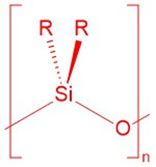
\includegraphics[width=0.2\textwidth]{2024/Abbildungen/Silicium/(R2SiO)n.png}
\end{figure}
1,5 P.}{5cm}




Ausgangsstoffe für die Silikon-Synthese sind Silicium und Methylchlorid (\ce{CH3Cl}). Bei 300\thinspace °C werden diese an einem Kupfer-Katalysator im sogenannten \textsc{Müller-Rochow}-Prozess zu Chlormethylsilanen, Derivaten von Monosilan  (\ce{SiH4}), umgesetzt. 

\enumaufgabe{\operator{Gib} die Summenformel aller möglichen  Chlormethylsilane, die beim \textsc{Müller-Rochow}-Prozess entstehen können, \operator{an}.} 
\solution{\ce{CH3SiCl3}, \ce{(CH3)2SiCl2}, \ce{(CH3)3SiCl}\\
je 0,5 P. jede falsche -0,5 P.; min. 0 P.\\
Insg. 1,5 P.}{2cm}


Durch vollständige Hydrolyse der Chlormethylsilane bilden sich Silanole, die im weiteren Verlauf spontan zu Silikonen kondensieren. 
Gegeben ist folgender Ausschnitt eines Silikons als Kondensationsprodukt von vier Silanolmolekülen: 


\begin{figure}[H]
    \centering
    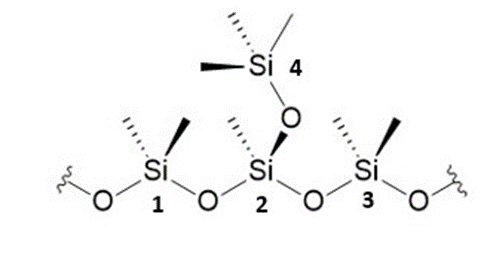
\includegraphics[width=0.4\textwidth]{2024/Abbildungen/Silicium/Silikon.png}
\end{figure}

\newpage

\enumaufgabe{\operator{Gib} die Struktur der Silanole \textbf{1}, \textbf{2}, \textbf{3} und \textbf{4}, welche zusammen zu dem Ausschnitt des Silikons reagieren, in Form einer Summenformel \operator{an}.} 
\solution{
\textbf{1} und \textbf{3}: \ce{(CH3)2Si(OH)2}\\
\textbf{2}: \ce{CH3Si(OH)3}\\
\textbf{4}: \ce{(CH3)3SiOH}\\
je 1 P. => 4 P.}{2cm}

\subsection{Rein oder nicht rein – das ist hier die Frage} 
Nicht nur in Kunststoffen wie den Silikonen hat sich Silicium unverzichtbar gemacht, sondern auch in der Halbleiterindustrie. So ist hochreines monokristallines Silicium das Ausgangsmaterial in der Halbleitertechnik. Der Weg dorthin ist allerdings lang und mühsam. 
Der erste Schritt ist die Gewinnung von Rohsilicium durch die Reduktion von \ce{SiO2} mit Koks bei Temperaturen von 2000\thinspace°C. 
\enumaufgabe{\operator{Stelle} die ausgeglichene Reaktionsgleichung zur Herstellung von Rohsilicium \operator{auf}.}
\solution{
\ce{SiO2 + 2 C -> Si + 2 CO}\\
0,5 P. jeweils für Produkte, Edukte und Stöchiometrie; insg. 1,5 P. }{3cm}
Das Rohsilicium wird im \textsc{Siemens}-Prozess zu polykristallinem Silicium umgewandelt. Bei dem Verfahren wird mithilfe einer Grundchemikalie zunächst ein Halogensilan gebildet. 
\enumaufgabe{\operator{Stelle} die Reaktionsgleichung des \textsc{Siemens}-Prozesses \operator{auf}. \\Hinweis: Es reagiert ein Äquivalent \ce{Si} mit drei Äquivalenten der Grundchemikalie.} 
\solution{\ce{Si + 3 HCl -> SiCl3H + H2} 2 P. }{3.5cm}
Dabei handelt es sich um eine Transportreaktion. Das heißt, dass das in Rohsilicium enthaltene Silicium in einer exothermen Reaktion in das Halogensilan überführt wird. Daraufhin wird das Gas an Stäben aufgefangen und bei der Rückreaktion scheidet sich Silicium ab. Im Ausgangsstoff enthaltene Verunreinigungen reagieren nicht und bleiben zurück. 

\newpage

\enumaufgabe{\operator{Begründe} ob die Hin- oder Rückreaktion bei höherer Temperatur abläuft.}
\solution{Es ist eine exotherme Reaktion, weshalb nach dem Prinzip von Le Chatilier (1 P.)  das GGW bei erhöhter Temperatur Richtung Edukte geschoben wird. Die Rückreaktion läuft damit bei höherer Temperatur ab. (1 P.)   
Alternative Erklärung: Die Rückreaktion muss bei höherer Temperatur ablaufen, da der Anteil an gasförmigen Molekülen auf der Eduktseite größer ist. Deshalb ist die Rückreaktion entropisch begünstigt  (1 P.) und das GGW verschiebt sich mit höher Temperatur zum Edukt (1 P.). \\
2 P.}{4cm}
\enumaufgabe{\operator{Nenne} drei Voraussetzungen, die eine Reaktion erfüllen muss, um als Transportreaktion genutzt werden zu können.} 
\solution{
z.B.\\
Transportmittel muss gasförmig sein.\\
Gasphasenkomplex/Reaktionsprodukt  muss gasförmig sein. \\
Ausgangsstoff muss flüssig oder fest sein.\\
Verunreinigungen dürfen nicht mit Transportmittel reagieren, zumindest nicht in ähnlicher Weise wie der zu transportierende Stoff.\\
Chemisches GGW darf nicht „extrem“ liegen, d.h. Richtung der Reaktion muss sich durch moderate Temperaturänderungen umkehren lassen.\\
je 1 P. insg. 3 P.}{5cm} 
Um das erhaltene polykristalline Silicium in monokristallines Silicium zu überführen, nutzt man entweder das \textsc{Czochralski}- oder das Zonenschmelzverfahren. Letzteres beruht darauf, dass sich entlang eines Stabs bestehend aus polykristallinem Silicium eine heiße Schmelzzone bewegt. Die wieder erkaltete Schmelze weist ein einheitliches Kristallgitter (monokristallin) auf, während sich die Verunreinigungen am Stabende anlagern und dort abgeschnitten werden können. 
\enumaufgabe{\operator{Kreuze an}, welche Triebkraft dem Zonenschmelzverfahren zugrunde liegt.} 

\begin{tabularx}{\textwidth}{|X|C{1.5cm}|}\hline
    Die Verunreinigungen verklumpen in der Hitze zu großen Clustern, die durch Konvektionsströme ans Stabende gedrückt werden.  & \emptybox \\\hline
    Die Verunreinigungen lösen sich in der Schmelze und wandern deshalb mit der Schmelze mit.	& \solutiontext{\checkedbox}{\emptybox} \\\hline
    In der Hitze ist die Reibung so groß, dass sich die Verunreinigungen elektrisch aufladen und an das Stabende elektrostatisch angezogen werden. 	& \emptybox \\\hline
    Sobald die Verunreinigungen durch die Hitze aus dem Kristallgitter freigesetzt wurden, wandern sie aufgrund der Erdanziehungskraft ans Stabende. & \emptybox \\\hline
\end{tabularx}
\solutiontext{1 P.}{}\\
\solutiontext{$\sum$ 24,5 P}{}
\end{document}